\section{Modality Transformation}
	\label{sec:mod}
Modality transformation refers to the steps taken to convert the data from a source mode to a target mode. The purpose of such a transformation is to exploit the knowledge present in pre-trained models in the target mode to allow for easy classification. In this section, we describe the process of modality transformation on the example of pressure sensor data.

\begin{figure}
	\centering
		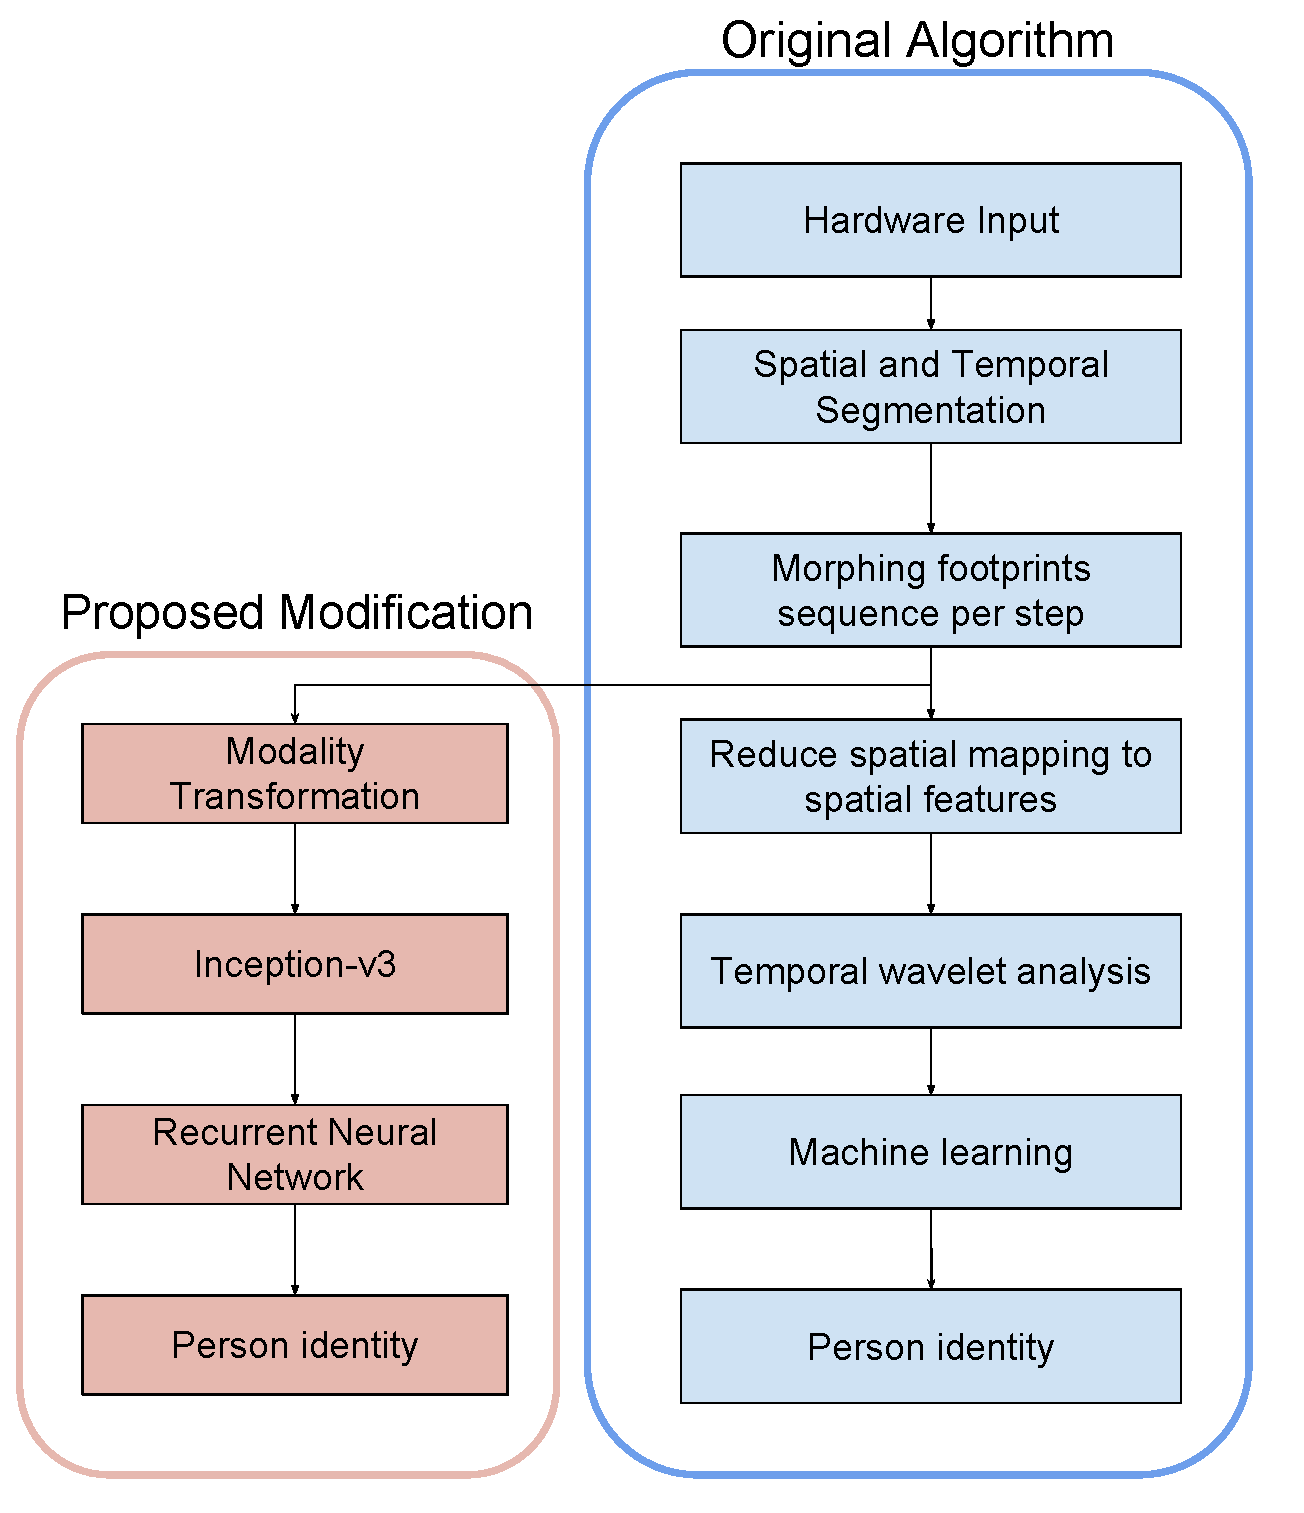
\includegraphics[height=6cm]{./figures/Flowchart.pdf}
	\caption{Original and proposed algorithm flow chart.}
	\label{fig:flowchart}
\end{figure}

%
%raw values
In our specific case, the modality transformation of the raw data from sensors constitute the steps to convert the sensor mode into the visual mode in the form of images. The raw data from the sensor is a temporal sequence of $120 \times 54$ 2-dimensional pressure mappings. For the force-sensitive resistor fabric sensor, every sensing point's value is essentially the voltage potential measurement that is related to the pressure. We transfer these values linearly into a gray-scale color map, in which each pixel represents a sensing point, and brighter color corresponds to higher pressure. A complete step is a sequence of such pressure mapping frames; every frame corresponds to the moment of a step as shown in Fig. \ref{fig:step_frames}(a). The number of frames which comprise the entire step varies among people. Thus, it is important to segment each step along temporal dimension and find the individual moments for each step. It is noteworthy that, the idea of modality transformation is not limited to pressure data. For other matrix-sensors, a similar modality transformation strategy can be applied. The main idea of this paper is that after such a modality transformation, it is possible to apply transfer learning on the transformed data.



%preproceesing
The modality transformation starts with the pre-processing of the raw data. Here, we first separate the steps from the background noise by converting each frame into a binary frame and applying an adaptive threshold. For the threshold, we sort the pixel values of the frame into a 10-bin histogram, and the threshold is decided as the center value of the next bin of the highest count bin.  However, this binarization process can be omitted for other pressure sensor data.

%bounding box
Next, we find the largest bounding box of all frames which encloses each individual step. It is, therefore, ensured that all the moments belonging to a same step will fit into that enclosing bounding box. Since, the bounding box is dynamically calculated for a step, the size of the enclosing box is different for different steps. However, within one step, all the moments are captured and extracted using the same sized bounding box. For the general modality transfer we suggest a position normalization in a similar manner, i.e., either cutting irrelevant parts with a bounding box or setting the center of the images to the mean position over all frames.
%ways of finding the images

There can be many ways to convert the data from the source mode to a visual imagery mode. This depends on a number of factors; the dimensionality, range, heterogeneity or homogeneity, volume, noisiness. Ideally the best way is the one which transforms the source mode data into a form as close as possible to the target mode on which the CNN has been trained. In the following, we describe three ways in which we extract the images after fitting the bounding box. 

The transformation on the sensor data can be done with three strategies: max-frame, averaging, sequential analysis, giving us three possible images per data sequence (per step). 

For the first strategy, we capture the maximum frame out of the frame sequence of each sample, which corresponds to the frame with highest value of pixel sum, then convert it into the respective image and label it with the class ID. As shown in Fig. \ref{fig:step_frames} (the frame with red bounding box), in our dataset, we obtain one such image for every step, hence, in total we have 529 such images. 

For the second strategy, we average over all the frames in the sequence of a single sample and generate the corresponding image with averaged pixel values. This is visualized for footstep data in Fig. \ref{fig:step_frames}(b). This averaged frame carries the temporal information from all the moments of the step and should be more effective than the maximum frames for classification. 

For the third strategy, we use all the frames which form a temporal sequence of a step within each sample and transform them into the images. The sequence of frames capturing the moments of a single step are shown in Fig. \ref{fig:step_frames}. This carries the original raw values at each frame and provides more granularity than previous approaches for the feature set calculation. 

	